\documentclass[a4]{beamer}
\usepackage{amssymb}
\usepackage{graphicx}
\usepackage{subfigure}
\usepackage{newlfont}
\usepackage{amsmath,amsthm,amsfonts}
%\usepackage{beamerthemesplit}
\usepackage{pgf,pgfarrows,pgfnodes,pgfautomata,pgfheaps,pgfshade}
\usepackage{mathptmx}  % Font Family
\usepackage{helvet}   % Font Family
\usepackage{color}

\mode<presentation> {
 \usetheme{Default} % was Frankfurt
 \useinnertheme{rounded}
 \useoutertheme{infolines}
 \usefonttheme{serif}
 %\usecolortheme{wolverine}
% \usecolortheme{rose}
\usefonttheme{structurebold}
}

\setbeamercovered{dynamic}

\title[MathsCast]{MathsCast Presentations \\ {\normalsize Standard Normal Distribution}}
\author[Kevin O'Brien]{Kevin O'Brien \\ {\scriptsize kevin.obrien@ul.ie}}
\date{Summer 2011}
\institute[Maths \& Stats]{Dept. of Mathematics \& Statistics, \\ University \textit{of} Limerick}

\renewcommand{\arraystretch}{1.5}


%------------------------------------------------------------------------%
\begin{document}


\frame{
\frametitle{MA4413 Autumn 2008 paper}
A model of an on-line computer system gives a mean times to retrieve a record from a direct access storage system device of 200 milliseconds, with a standard deviation of 58 milliseconds. If it can assumed that the retrieval times are normally distributed:

\begin{itemize}
\item[(i)] What proportion of retrieval times will be greater than 75 milliseconds?
\item[(ii)] What proportion of retrieval times will be between 150 and 250 milliseconds?
\item[(iii)] What is the retrieval time below which 10\% of retrieval times will be?
\end{itemize}

}
%---------------------------------------------%

\frame{
\frametitle{Normal Distribution}

\begin{center}
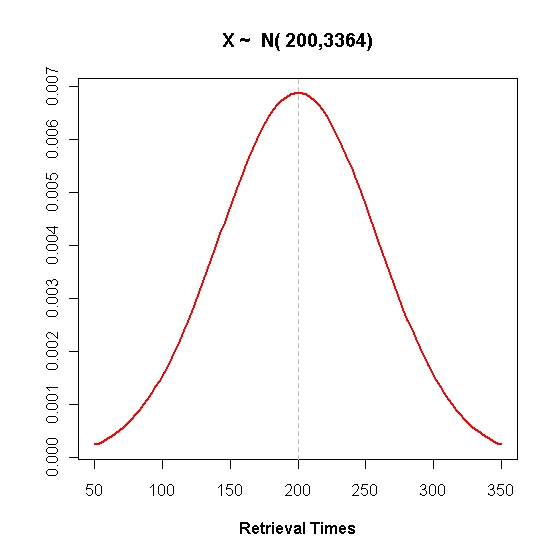
\includegraphics[scale=0.40]{images/5BNormal1}
\end{center}

}
%-----------------------------------------------------%


\frame{
\frametitle{MA4413 Autumn 2008 paper (part 1)}
What proportion of retrieval times will be greater than 75 milliseconds?\\ \bigskip

\begin{itemize}
\item Let X be the retrieval times, with $X \sim \mbox{N}(200,58^2)$.\\
\item The first question asks us to find $P( X \geq 75)$. \\
\item First compute the z score.
\[ z_o =  {x_o - \mu \over \sigma} = {75 - 200 \over 58}  = -2.15 \]
\end{itemize}
}

\frame{
\frametitle{Normal Distribution}

\begin{center}
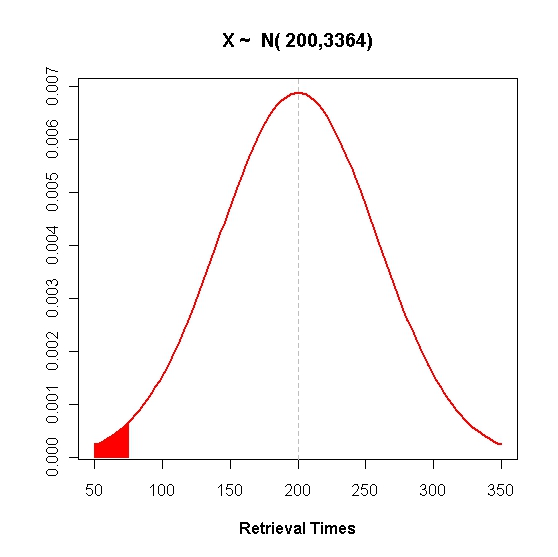
\includegraphics[scale=0.40]{images/5BNormal2}
\end{center}

In this case, the probability of interest $P(X\geq 75)$, is represented by the white area under the curve.

}

\frame{
\frametitle{MA4413 Autumn 2008 paper (part 1)}
\begin{itemize}
\item We can say
\[ P( X \geq 75) = P( Z \geq -2.15)\]
\item Using symmetry rule and complement rule
\[ P( Z \geq -2.15) = P( Z \leq 2.15) = 1- P( Z \geq 2.15)\]
\item From tables $P( Z \geq 2.15) = 0.0158$
\item Therefore $P( Z \leq 2.15) = 0.9842$ 
\item Furthermore $P( X \geq 75) = \boldsymbol{0.9842}$ [Answer].
\end{itemize}
}
\frame{
\frametitle{Normal Distribution}

\begin{center}
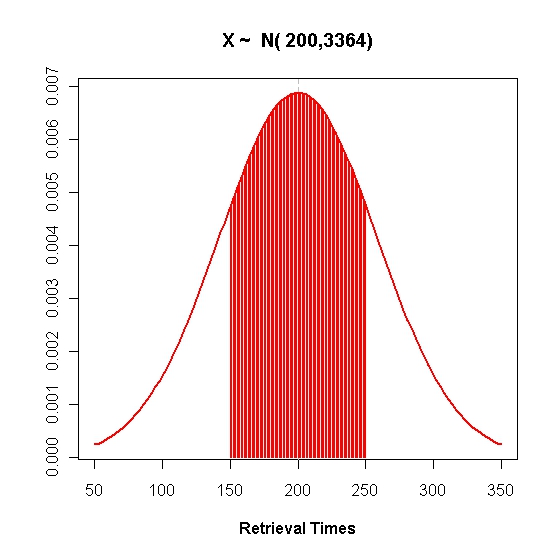
\includegraphics[scale=0.40]{images/5BNormal3}
\end{center}

}
%---------------------------------------------%
\frame{
\frametitle{MA4413 Autumn 2008 paper (part 2)}
\begin{itemize}
\item What proportion of retrieval times will be between 150 and 250 milliseconds?
\item Find $P(150 \leq X \leq 250)$
\item Use the `Too Low / Too High ' approach.
\item Too low $P( X \leq 150)$
\item Too high $P( X \geq 250)$
\item Find the z-scores for each.
\[ z_{150} =  {150 - 200 \over 58}  = -0.86 \]
\[ z_{250} =  {250 - 200 \over 58}  = 0.86 \]
\end{itemize}
}
%---------------------------------------------%
\frame{
\frametitle{MA4413 Autumn 2008 paper (part 2)}
\begin{itemize}
\item We can now say
\[ 1. P( X \leq 150) = P( Z \leq -0.86)\]
\[ 2. P( X \geq 250) = P( Z \geq 0.86)\]
\item By symmetry rule, $P( Z \leq -0.86) = P( Z \geq 0.86)$
\[ P( X \leq 150) =  P( X \geq 250) \]
\item Let's compute $P( X \geq 250)$. Using tables 
\[P( X \geq 250) = P( Z \geq 0.86) = 0.1949 \]
\end{itemize}
}
%---------------------------------------------%
\frame{
\frametitle{MA4413 Autumn 2008 paper (part 2)}
\begin{itemize}
\item Too high: $P( X \geq 250) = 0.1949 $
\item Too low:  $P( X \leq 150) = 0.1949 $
\item Probability of being inside interval: 

\[ P(150 \leq X \leq 250) = 1- [ P( X \leq 150) + P( X \geq 250)] \]

\item $P(150 \leq X \leq 250) = 1- [ 0.1949 + 0.1949 ] = \boldsymbol{0.6102}$

\end{itemize}
}
%---------------------------------------------%
\frame{
\frametitle{MA4413 Autumn 2008 paper (part 3)}
\begin{itemize}
\item What is the retrieval time below which 10\% of retrieval times will be?
\item Find $A$ such that $P(X \leq A) = 0.10$.
\item What z-score would correspond to $A$? Lets call it $z_A$.
\item $P(Z  \leq z_A) = 0.10$
\item Remark: $z_A$ could be negative.
\item Using symmetry $P(Z \geq -z_A) = 0.10$
\item Remark: $-z_A$ could be positive.
\end{itemize}
}

\frame{
\frametitle{Normal Distribution}

\begin{center}
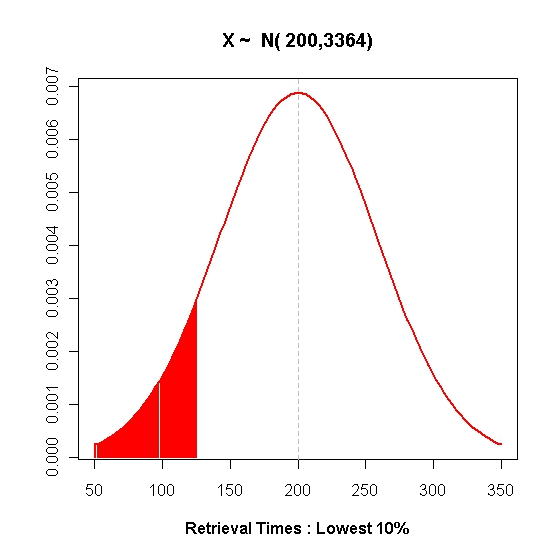
\includegraphics[scale=0.40]{images/5BNormal4}
\end{center}

}
%---------------------------------------------%
\frame{
\frametitle{MA4413 Autumn 2008 paper (part 3)}
\begin{itemize}
\item Use the Murdoch Barnes tables to get an approximate value for $-z_A$.
\item The nearest value we can get is 1.28. ( $P( Z \geq 1.28) = 0.1003$ ).
\item If $-z_A = 1.28$, then $z_A=-1.28$
\item We can now say
\[ P(X \leq A) = P(Z \leq -1.28) \]

\end{itemize} 
}
%---------------------------------------------%
\frame{
\frametitle{MA4413 Autumn 2008 paper (part 3)}
\begin{itemize}
\item Necessarily $A$ and $Z_A$ are related by the standardization formula
\item Recall that $\mu = 200$ and $\sigma = 58$.
\[ -1.28  = {A - 200 \over 58} \]
\item Re-arranging ( multiply both sides by 58)
\[ -74.24  = A - 200 \]
\item Re-arranging again (Add 200 to both sides)
\[ 125.76 =  A \]
\end{itemize}
}
%---------------------------------------------%
\frame{
\frametitle{MA4413 Autumn 2008 paper (part 3)}
\begin{itemize}
\item Now we know the retrieval time below which 10\% of retrieval times will be.
\item $P(X \leq 125.76) = 0.10$ [Answer].
\end{itemize}
}

\end{document}
